\documentclass[a4paper,titlepage,11pt]{article}
\usepackage{a4wide}
\usepackage{fullpage}
\usepackage[utf8x]{inputenc}
\usepackage[slovene]{babel}
\selectlanguage{slovene}
\usepackage[toc,page]{appendix}
\usepackage[pdftex]{graphicx} % za slike
\usepackage{setspace}
\usepackage{color}
\usepackage{amsmath}
\usepackage[table]{xcolor}
\usepackage{tabularx}
\usepackage{float}
\usepackage{hhline}
\definecolor{light-gray}{gray}{0.95}
\usepackage{listings} % za vključevanje kode
\usepackage{hyperref}
\renewcommand{\baselinestretch}{1.2} % za boljšo berljivost večji razmak
\renewcommand{\arraystretch}{1.2}
\hyphenpenalty=10000
\newcolumntype{Y}{>{\centering\arraybackslash}X}
\usepackage[font=small, skip=11pt, hypcap=true]{caption}
\usepackage{indentfirst}
\setlength{\parskip}{11pt}
\usepackage{multirow}

\title{Temperaturna plošča}
\author{Rok Grmek, Matej Klemen}
\date{3. november 2017}

\begin{document}

\maketitle

\tableofcontents
\pagebreak

\section*{Uvod}

V okviru predmeta Porazdeljeni sistemi rešujeva problem temperaturne plošče. Na tem problemu bova tekom semestra spoznavala različne pristope za paralelno programiranje.

Problem temperaturne plošče je predstavljen s ploščo, ki je na treh straneh (zgoraj, levo in desno) segreta na 100 °C, na spodnji stranici pa ohlajena na 0 °C. Zanima nas, kako se v takem primeru toplota porazdeli po plošči (primer porazdelitve temperature je viden na sliki \ref{slika-primer-temperaturne-plosce}).

\begin{figure}[H]
\begin{center}

\includegraphics[scale=0.6]{primer-temperaturne-plosce.png}
\caption{Primer temperaturne plošče, kjer rdeča barva prikazuje najvišjo, temno modra barva pa najnižjo temperaturo.}
\label{slika-primer-temperaturne-plosce}
\end{center}
\vspace{-25pt}
\end{figure}

Iskala bova stacionarno rešitev enačbe \(\nabla^2 W = f(x, y)\), pomagala pa si bova z metodo končnih diferenc. Ploščo bova najprej razdelila na mrežo točk in posameznim točkam določila začetne vrednosti. Nato bova v vsaki točki izračunala novo temperaturo na podlagi sosednjih točk. Postopek računanja novih točk se bo ponavljal, dokler rešitev ne skonvergira.

\pagebreak

\section{Serijski algoritem}

\subsection{Opis implementacije}

Program ima dva načina delovanja. Če je definirana vrednost \textit{TIME\_MEASUREMENTS}, se bo program za podane argumente večkrat izvedel in izračunal nekaj uporabnih statistik. Ta način je namenjen predvsem opazovanju časa izvajanja programa. Sicer pa se bo program izvedel 1-krat in na koncu vizualiziral porazdelitev temperature na plošči. V nadaljevanju je opisan slednji način izvajanja, celotno delovanje programa pa je predstavljeno tudi z diagramom zaporedja, vidnim na sliki \ref{slika-diagram-zaporedja}.

\begin{figure}[H]
\begin{center}
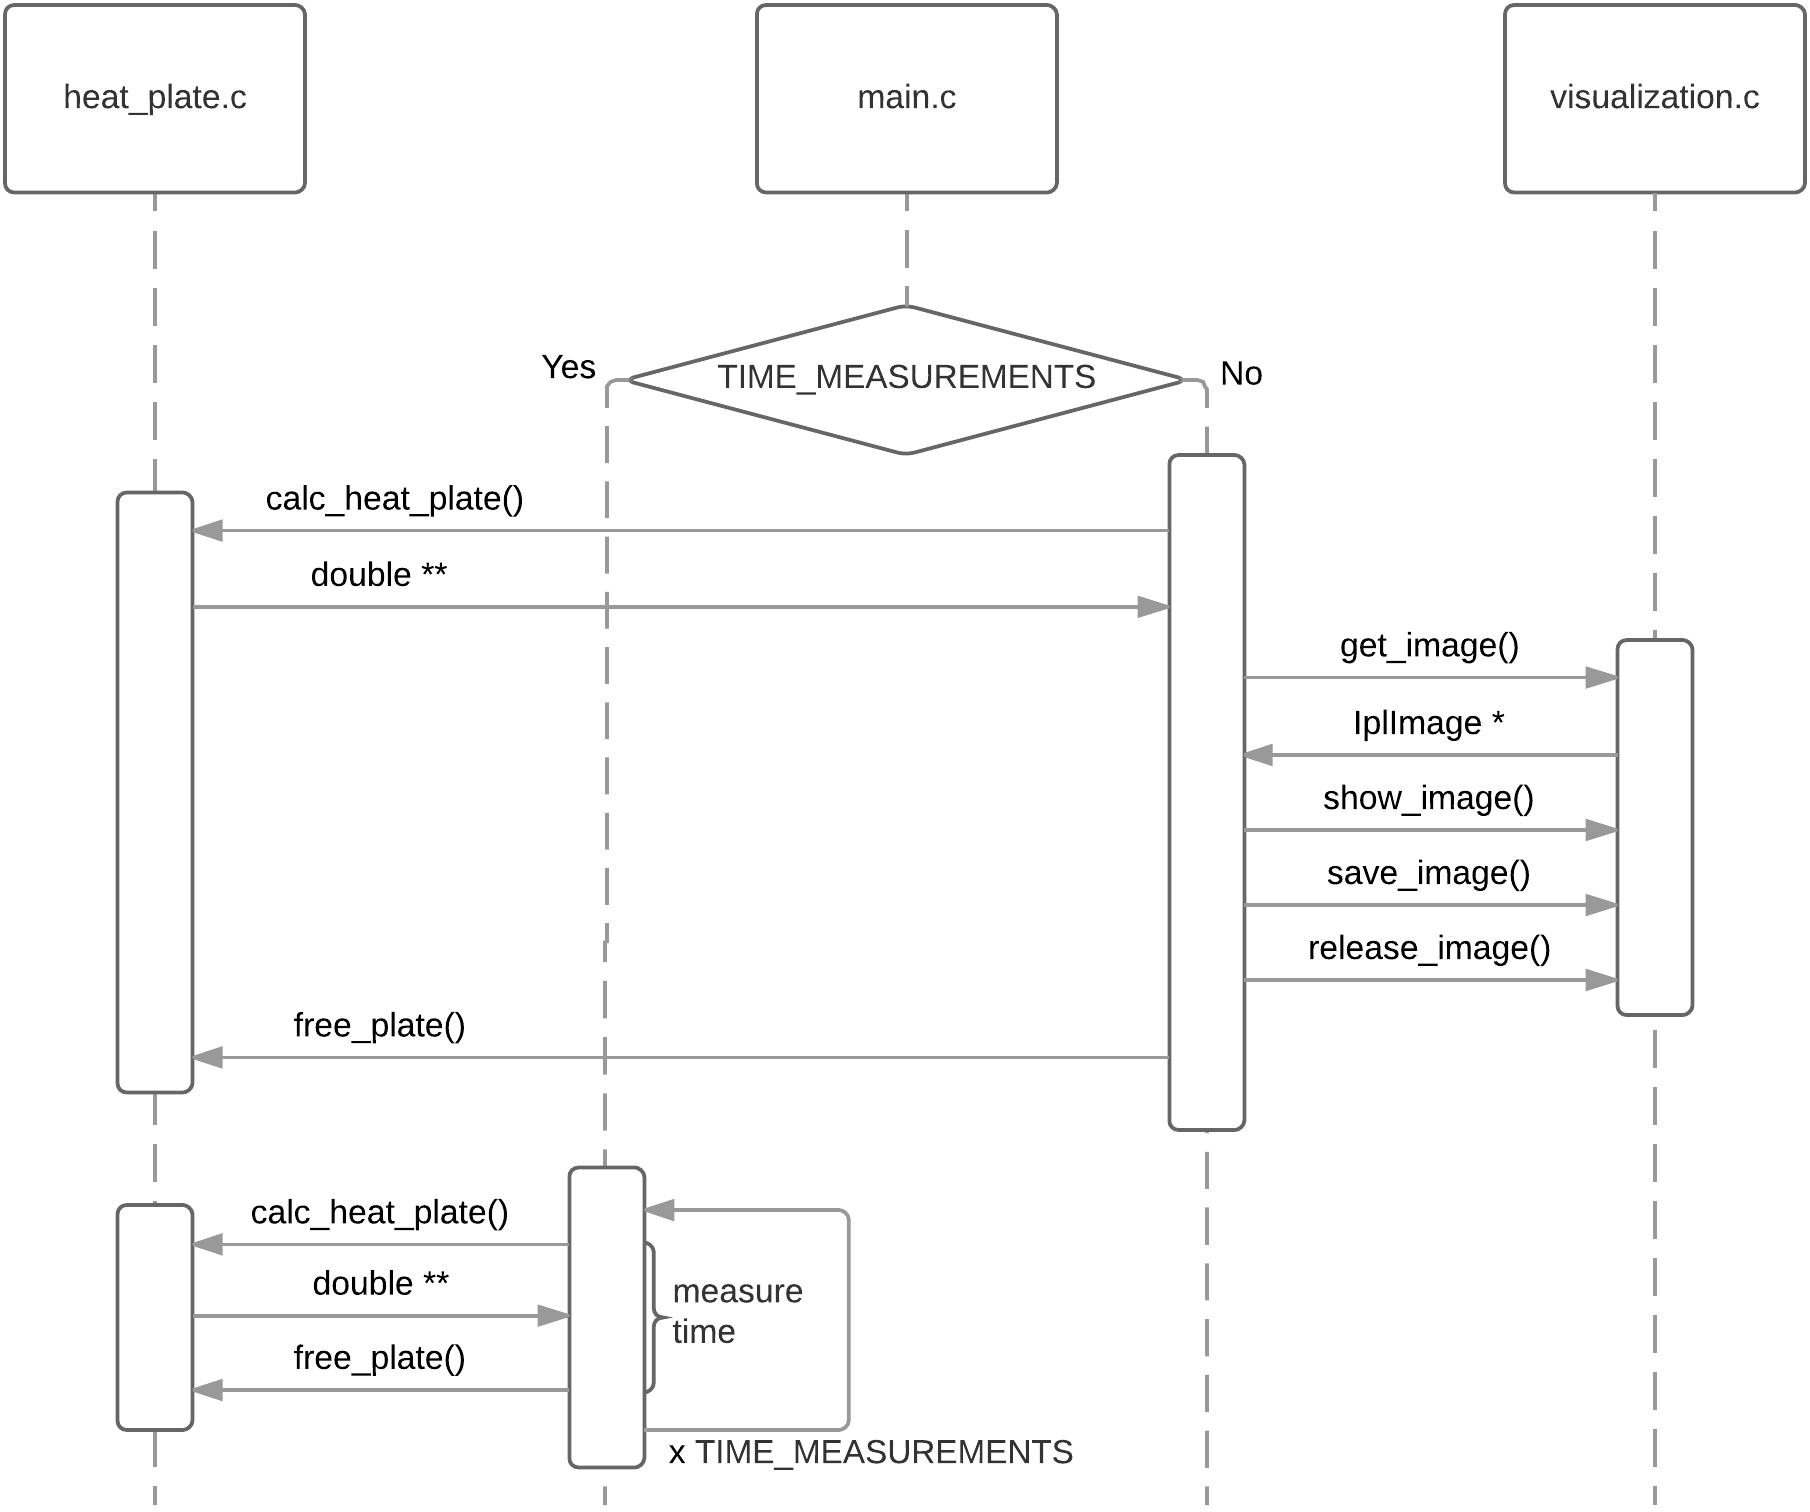
\includegraphics[scale=0.8]{diagram-zaporedja.png}
\caption{Diagram zaporedja, ki prikazuje delovanje programa.}
\label{slika-diagram-zaporedja}
\end{center}
\vspace{-25pt}
\end{figure}

Algoritem sprejme 3 argumente: višino plošče, širino plošče in mejno razliko med dvema iteracijama (v nadaljevanju označeno z \(\varepsilon\)), na podlagi katere se zaključi računanje. Plošči, ki jo določata vnešena višina in širina, algoritem na vseh štirih stranicah doda pas širine 1, ki služi za nastavljanje robnega pogoja temperature. Novi dimenziji sta torej:
\begin{equation}
vi\breve{s}ina := vi\breve{s}ina + 2
\end{equation}
\begin{equation}
\breve{s}irina := \breve{s}irina + 2
\end{equation}
Na začetku se alocirata dve tabeli dimenzij $ vi\breve{s}ina \times \breve{s}irina$. Ena predstavlja trenutno stanje plošče, druga pa stanje plošče v prejšnji iteraciji. Alokaciji sledi inicializacija plošče - trem stranicam (levi, desni, zgornji) algoritem nastavi temperaturo na 100 °C, eni (spodnji) pa na 0 °C. Vsem ostalim celicam plošče se zaporedno (\textit{od zgoraj navzdol, od leve proti desni}) dodeli povprečje leve sosednje, zgornje sosednje, povsem desne ter povsem spodnje celice plošče. Eno izmed plošč algoritem izbere kot ploščo trenutnega, drugo pa kot ploščo prejšnjega stanja.
\indent \par Nato sledi glavna zanka. V vsaki iteraciji gre algoritem skozi ``dinamične'' celice plošče (celice, ki niso del katerega izmed robov plošče) in za vsako tako celico c[i][j] v \textit{i}-ti vrstici in \textit{j}-tem stolpcu po naslednji formuli izračuna novo temperaturo:
\begin{equation}
c[i][j] := \frac{c'[i - 1][j] + c'[i][j - 1] + c'[i][j + 1] + c'[i + 1][j]}{4},
\end{equation}
kjer $c'[i][j]$ predstavlja temperaturo celice v \textit{i}-ti vrstici in \textit{j}-tem stolpcu v prejšnji iteraciji. Ob vsakem izračunu nove temperature algoritem izračuna še absolutno razliko med trenutno (novo) in prejšnjo temperaturo ter jo v primeru, da je to v trenutni iteraciji največja izračunana absolutna razlika temperatur, shrani. Ob koncu iteracije algoritem zamenja vlogi plošč (tista, ki je do sedaj predstavljala prejšnje stanje plošče, bo v naslednji iteraciji vsebovala novo stanje plošče in obratno), pred prehodom v naslednjo iteracijo pa preveri, če je temperaturna razlika v tej iteraciji že manjša od \(\varepsilon\) (v takem primeru se računanje zaključi).

Na koncu algoritem izpiše število izvedenih iteracij in zažene vizualizacijo končnega stanja temperaturne plošče. O vizualizaciji temperaturne plošče pa je več napisano v naslednjem poglavju.

\subsection{Uporabljene knjižnice}

Za vizualizacijo temperaturne plošče uporabljava knjižnico \textit{OpenCV}. Najprej se pripravi prazna slika (\textit{cvCreateImage}) z dimenzijami naše plošče, nato pa se za vsako točko na plošči pretvori temperaturo v 3 8-bitne kanale (rdeča, zelena, modra) in vrednosti prepiše na sliko. Če slika z največjo stranico presega \textit{MAX\_SIZE}, potem se jo še pomanjša (\textit{cvResize}). Pripravljeno sliko se prikaže (\textit{cvShowImage}) v oknu (\textit{cvNamedWindow}, \textit{cvMoveWindow}, \textit{cvResizeWindow}) in shrani na disk (\textit{cvSaveImage}). Na koncu se le še sprosti zaseden pomnilnik (\textit{cvReleaseImage}). Primer vizualizacije je viden na sliki \ref{slika-primer-temperaturne-plosce}.

\subsection{Rezultati}

Program je bil testiran na sistemu, katerega specifikacije so navedene v tabeli \ref{tabela-specifikacije}. Da bi k izmerjenemu času čim manj pripomogli stroški režije operacijskega sistema, je bil sistem med testiranjem minimalno obremenjen z drugimi procesi.
\begin{table}[H]
\begin{center}
\caption{Specifikacije testnega sistema.}
\label{tabela-specifikacije}
\begin{tabularx}{\textwidth}{|YY|}
\hhline{==}
Procesor: & Intel Core i5-4210U\tabularnewline
Frekvenca procesorja: & 1.70GHz \tabularnewline
Število jeder: & 2 \tabularnewline
Maksimalno število niti: & 4 \tabularnewline
Velikost predpomnilnika: & 3MB \tabularnewline
Velikost in tip glavnega pomnilnika: & 16GB DDR3 \tabularnewline
Grafična kartica: & NVIDIA GeForce 820M 2GB DDR3 \tabularnewline
Operacijski sistem: & Ubuntu 16.04 \tabularnewline
\hhline{==}
\end{tabularx}
\end{center}
\vspace{-25pt}
\end{table}

Pri testiranju sva se omejila na fiksno vrednost \(\varepsilon = 0,01\) in na plošče kvadratne oblike, spreminjala pa sva zgolj velikost stranice. Za vsako izbrano velikost sva algoritem 100-krat zagnala in vsakič izmerila čas izvajanja. Iz meritev sva nato izračunala povprečni čas izvajanja in standardno napako (ta predstavlja razpršenost meritev okrog povprečnega časa). Rezultati so navedeni tabelarično v tabeli \ref{tabela-rezultati-1} in z grafom, prikazanim na sliki \ref{graf-rezultati-1}.

\begin{table}[H]
\begin{center}
\caption{Povprečni čas izvajanja programa in standardna napaka v odvisnosti od velikosti stranice.}
\label{tabela-rezultati-1}
\begin{tabularx}{\textwidth}{|YYY|}
\hhline{===}
Velikost stranice [št. točk] & Povprečni čas izvajanja [s] & Standardna napaka [s] \tabularnewline
\hhline{===}
100 & 0,250 & 0,000 \tabularnewline
200 & 0,965 & 0,001 \tabularnewline
400 & 3,877 & 0,003 \tabularnewline
800 & 15,516 & 0,006 \tabularnewline
1600 & 62,272 & 0,062 \tabularnewline
\hhline{===}
\end{tabularx}
\end{center}
\vspace{-25pt}
\end{table}

\begin{figure}[H]
\begin{center}
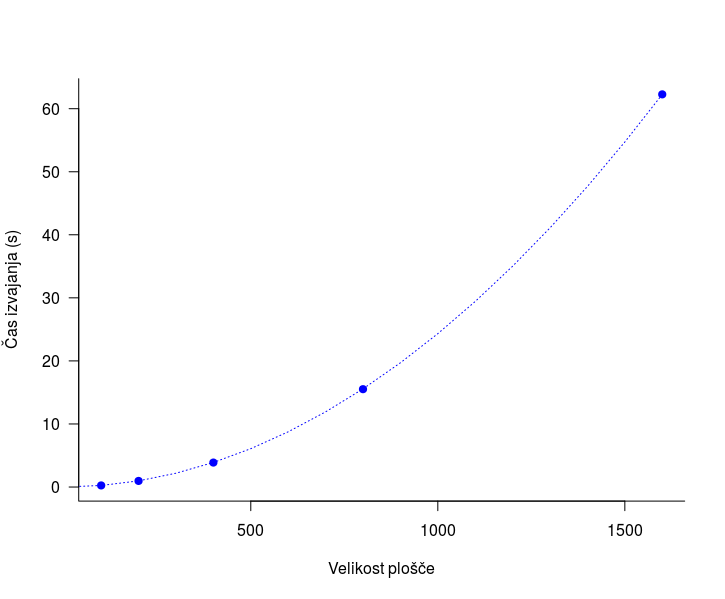
\includegraphics[scale=0.55]{graf-rezultati-1.png}
\caption{Graf, ki prikazuje povprečni čas izvajanja programa v odvisnosti od velikosti stranice.}
\label{graf-rezultati-1}
\end{center}
\vspace{-25pt}
\end{figure}

Iz rezultatov je vidno, da je povprečni čas izvajanja kvadratno odvisen od velikosti stranice plošče, kar ustreza tudi teoretični časovni zahtevnosti \(O(k \cdot h \cdot w)\), kjer je \textit{k} število iteracij, \textit{h} višina, \textit{w} pa širina plošče. V našem primeru je namreč število iteracij konstantno (določeno z \(\varepsilon\)) in velja zveza \(h=w\). Točke na grafu se zelo lepo prilegajo funkciji \(t(x) = 2,432 \cdot 10^{-5} \cdot x^{2}\), iz te pa lahko razberemo, da algoritem na testnem sistemu potrebuje približno \(2,432 \cdot 10^{-5}\) s za izračun posamezne točke (v vseh iteracijah skupaj).

\pagebreak

\section{Paralelizacija s knjižnico ``Pthreads''}
\label{poglavje-pthreads}

\subsection{Ideja paralelizacije} \label{poglavje-ideja-paralelizacije-2}

Do vključno inicializacije plošč poteka vse enako kot v serijskem algoritmu, za tem pa se delo razdeli med \textit{NUM\_THREADS} niti. Vsaka nit v posamezni iteraciji izračuna svoj delež vrstic. Pred računanjem se meje vrstic določijo na podlagi spodnjih enačb (\textit{index} predstavlja zaporedno številko niti iz intervala $\left[0, NUM\_THREADS - 1\right]$, ki jo dobi posamezna nit podano kot argument).
\begin{equation}
spodnja \ meja := 1 + \left \lfloor{\frac{index \cdot (h - 2)}{NUM\_THREADS}}\right \rfloor
\end{equation}
\begin{equation}
zgornja \ meja := 1 + \left \lfloor{\frac{(index+1) \cdot (h - 2)}{NUM\_THREADS}}\right \rfloor
\end{equation}
V zgornjih enačbah $(h - 2)$ predstavlja število vrstic, katerih temperatura ni fiksno nastavljena. Te razdeliva kar se da enakomerno med niti, na koncu pa mejam še prištejeva 1, saj je temperatura prve vrstice fiksno nastavljena na 100 °C in se računanje začne v drugi vrstici. V takem primeru delitve se število dodeljenih vrstic med posamenzimi nitmi razlikuje za kvečjemu eno vrstico.

Ko niti poračunajo svoj del plošče, morajo počakati na preostale niti, saj je nadaljnje izvajanje programa odvisno od izračunov vseh niti v trenutni iteraciji. To je doseženo s postavitvijo t.i. prepreke (angl. \textit{barrier}), ki nitim ne pusti opravljati nadaljnjega dela, dokler vse niti ne pridejo do mesta, kjer je postavljena.

Sledi postopek sinhronizacije največje izračunane absolutne razlike temperature v trenutni iteraciji. Vsaka nit je ta podatek izračunala na svojem delu plošče in ga shranila globalno, v tem delu pa posamezna nit preveri, če so vsi izračunani lokalni maksimumi pod mejo \(\varepsilon\). V takem primeru se računanje zaključi, niti se združijo in program poteka od tu naprej enako kot pri serijskem algoritmu. V nasprotnem primeru se niti počakajo (še ena prepreka) in nato hkrati začnejo novo iteracijo.

\subsection{Rezultati} \label{poglavje-rezultati-2}

Program je bil testiran na istem sistemu (specifikacije so navedene v tabeli \ref{tabela-specifikacije}) in pri enakih pogojih kot serijski algoritem. Za fiksno vrednost \(\varepsilon = 0,01\) sva izmerila čase pri različnih velikostih plošče in za različno število niti. Rezultati so vidni v tabeli \ref{tabela-rezultati-2} in na grafu \ref{graf-rezultati-2}.

\begin{table}[H]
\begin{center}
\caption{Povprečni čas izvajanja paralelnega programa in standardna napaka glede na velikost stranice in število uporabljenih niti z uporabo knjižnice Pthreads.}
\label{tabela-rezultati-2}
\begin{tabularx}{\textwidth}{|YYYY|}
\hhline{====}
Število uporabljenih niti & Velikost stranice [št. točk] & Povprečni čas izvajanja [s] & Standardna napaka [s] \tabularnewline
\hhline{====}
\multirow{ 5}{*}{1}
& 100 & 0,253 & 0,000 \tabularnewline
& 200 & 0,974 & 0,000 \tabularnewline
& 400 & 3,890 & 0,002 \tabularnewline
& 800 & 15,935 & 0,071 \tabularnewline
& 1600 & 62,760 & 0,052 \tabularnewline
\hline
\multirow{ 5}{*}{2}
& 100 & 0,167 & 0,002 \tabularnewline
& 200 & 0,578 & 0,006 \tabularnewline
& 400 & 2,282 & 0,020 \tabularnewline
& 800 & 9,130 & 0,044 \tabularnewline
& 1600 & 35,545 & 0,030 \tabularnewline
\hline
\multirow{ 5}{*}{3}
& 100 & 0,199 & 0,000 \tabularnewline
& 200 & 0,729 & 0,000 \tabularnewline
& 400 & 2,740 & 0,000 \tabularnewline
& 800 & 10,778 & 0,002 \tabularnewline
& 1600 & 42,850 & 0,005 \tabularnewline
\hline
\multirow{ 5}{*}{4}
& 100 & 0,163 & 0,001 \tabularnewline
& 200 & 0,558 & 0,001 \tabularnewline
& 400 & 2,149 & 0,000 \tabularnewline
& 800 & 8,557 & 0,001 \tabularnewline
& 1600 & 33,917 & 0,005 \tabularnewline
\hline
\multirow{ 5}{*}{8}
& 100 & 0,212 & 0,000 \tabularnewline
& 200 & 0,680 & 0,001 \tabularnewline
& 400 & 2,414 & 0,001 \tabularnewline
& 800 & 8,874 & 0,003 \tabularnewline
& 1600 & 34,636 & 0,023 \tabularnewline
\hline
\hhline{====}
\end{tabularx}
\end{center}
\vspace{-25pt}
\end{table}

\begin{figure}[H]
\begin{center}
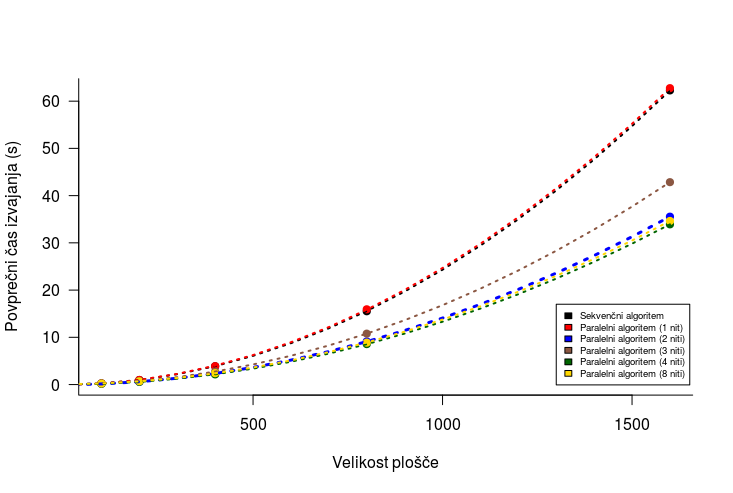
\includegraphics[scale=0.55]{graf-rezultati-2_1.png}
\caption{Povprečni čas izvajanja paralelnega programa glede na velikost plošče ob uporabi različnega števila niti (Pthreads).}
\label{graf-rezultati-2}
\end{center}
\vspace{-25pt}
\end{figure}

Za lažjo analizo meritev definiramo \textbf{faktor pohitritve} $S$ kot:
\begin{equation} \label{enacba-faktor-pohitritve}
S = \frac{T_s}{T_p},
\end{equation}
kjer je $T_s$ čas izvajanja sekvenčnega programa, $T_p$ pa čas izvajanja paralelnega programa. Največja dosežena pohitritev je bila 1,813-krat, in sicer v primeru štirih niti (toliko je tudi logičnih jeder na testnem sistemu). Ta pohitritev je sicer le malo boljša od tiste v primeru dveh niti, ampak je tak rezultat pričakovan, saj imamo le dve fizični jedri. ``Hyper-threading'' nam ne prinese bistvene pohitritve, saj je naše računanje zahtevno tudi iz vidika pomnilniških dostopov, tukaj pa si po dve niti delita eno fizično jedro, kar pomeni, da uporabljata tudi isti predpomnilnik in prihaja do številnih zgrešitev. Zanimiv je še primer treh niti, pri katerem dosežemo celo manjšo pohitritev kot v primeru dveh niti. To si lahko razlagamo tako. Naj bo hitrost posamezne niti enaka številu izračunanih celic plošče na enoto časa (merjeno v času, ko nit računa). Če primerjamo primer štirih niti s primerom dveh niti vidimo, da je hitrost posamezne niti manjša, ko uporabljamo štiri niti, ampak je čas, potreben za posamezno iteracijo v tem primeru vseeno manjši, ker imajo posamezne niti dodeljeno le četrtino (in ne polovico) plošče. V primeru treh niti je hitrost primerljiva s primerom štirih niti, ker si dve od treh niti delita eno fizično jedro in je skupna hitrost zaradi čakanja ob prepreki na koncu vsake iteracije odvisna od hitrosti najpočasnejše niti. Čas, potreben za posamezno iteracijo, pa je tukaj še večji od tistega v primeru dveh (in tudi štirih) niti, ker ima vsaka nit dodeljeno tretino plošče. Drugače povedano, ena od niti je hitrejša od ostalih dveh in zaradi enakomerne delitve dela prej konča z računanjem posamezne iteracije, nato pa neučinkovito čaka preostali dve niti. Tudi v primeru večjega števila niti (npr. 8) nam faktor pohitritve rahlo pada, saj čas izvajanja narašča še zaradi režije in preklapljanja med nitmi, hkrati pa že izkoriščamo vse razpoložljive vire sistema. Vse to je vidno tudi na grafu \ref{graf-rezultati-pohitritev-2}.

\begin{figure}[H]
\begin{center}
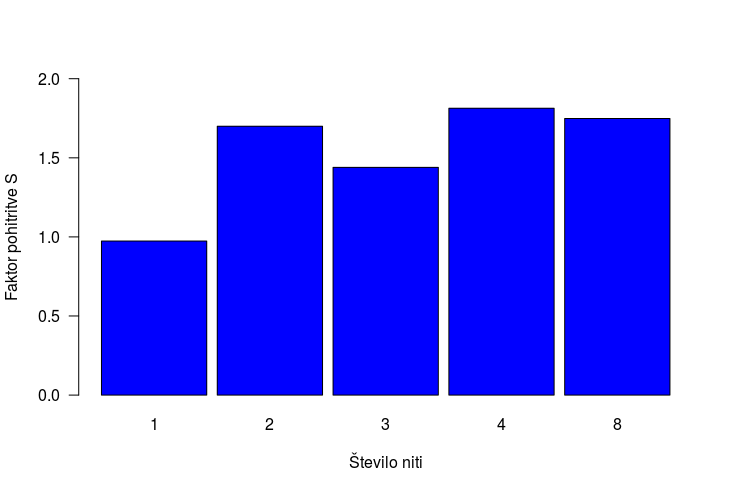
\includegraphics[scale=0.55]{graf-rezultati-2_2.png}
\caption{Faktor pohitritve v odvisnosti od števila uporabljenih niti za fiksno velikost plošče 800$\times$800 (Pthreads).}
\label{graf-rezultati-pohitritev-2}
\end{center}
\vspace{-25pt}
\end{figure}

Smiselno je preveriti še \textbf{učinkovitost} oziroma izkoristek uporabljenih niti, $E$, ki jo izračunamo kot:
\begin{equation} \label{enacba-ucinkovitost}
E = \frac{S_N}{N},
\end{equation}
kjer je $S_N$ faktor pohitritve in $N$ število niti. Učinkovitost je najboljša v primeru ene same niti (0,974). Rahlo slabšo, a še vedno zadovoljivo učinkovitost dosežemo tudi za dve niti (0,849), pri večjem številu niti pa ta precej pade, saj smo omejeni na zgolj dve fizični jedri. Učinkovitost v odvisnosti od števila niti je vidna na grafu \ref{graf-rezultati-ucinkovitost-2}.

\begin{figure}[H]
\begin{center}
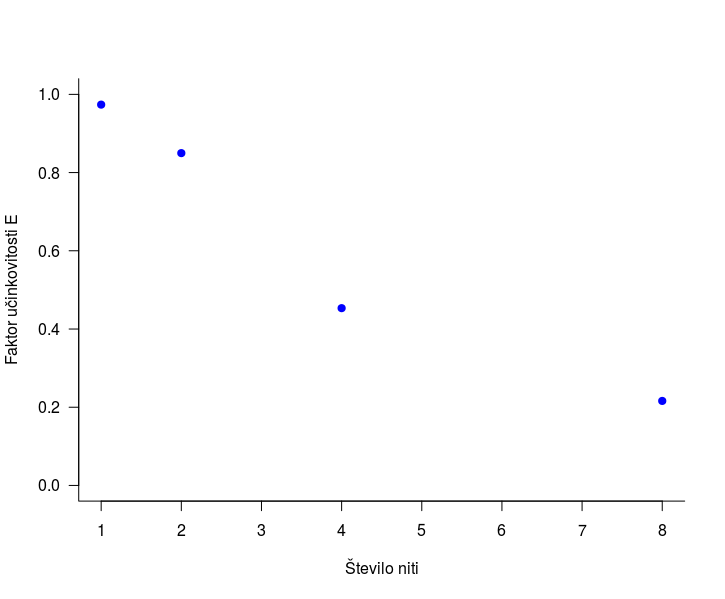
\includegraphics[scale=0.55]{graf-rezultati-2_3.png}
\caption{Učinkovitost v odvisnosti od števila uporabljenih niti za fiksno velikost plošče 800$\times$800 (Pthreads).}
\label{graf-rezultati-ucinkovitost-2}
\end{center}
\vspace{-25pt}
\end{figure}

\pagebreak

\section{Paralelizacija s knjižnico ``OpenMP''}
\label{poglavje-openmp}

\subsection{Ideja paralelizacije}
Paralelizacija poteka na podoben način kot paralelizacija s knjižnico Pthreads (za katero je ideja paralelizacije opisana v poglavju \ref{poglavje-ideja-paralelizacije-2}). Na začetku vsake iteracije se delo statično razdeli med vse niti - vsaka nit dobi $\frac{\breve{s}tevilo \ vrstic \ - \ 2}{\breve{s}tevilo \ niti}$ vrstic. Če $\breve{s}tevilo \ vrstic \ - \ 2$ ni deljivo s $\breve{s}tevilo \ niti$ (ostane $0 < r < \breve{s}tevilo \ niti$), potem se prvim $r$ nitim dodeli še po 1 vrstico.

Zatem vsaka nit poračuna svoj del plošče, na koncu pa niti sinhronizirajo maksimalne absolutne razlike med starimi in novimi temperaturami, ki so jih izračunale na svojem delu plošče v trenutni iteraciji. Če je največja izmed teh temperatur manjša od meje konvergence $\varepsilon$, se izračun konča, sicer pa se začne nova iteracija in ponovi postopek.

V primerjavi s paralelizacijo s knjižnico Pthreads je bilo tukaj potrebno manj dela. Če zanemarimo vključevanje knjižnice OpenMP in nastavitev števila niti, ki jih program uporablja, je bila paralelizacija dosežena zgolj z naslednjo vrstico:
\begin{lstlisting}
#pragma omp parallel for schedule(static) reduction(max: max_diff).
\end{lstlisting}
To navodilo prevajalniku pove, naj poskrbi, da se delo porazdeli tako, kot je bilo navedeno v prvem odstavku tega poglavja ter da se niti na koncu počakajo in sinhronizirajo svoje lokalne podatke.

\subsection{Rezultati}

Program je bil testiran na sistemu, opisanem v tabeli \ref{tabela-specifikacije}. Izmerjeni časi so zelo podobni časom, izmerjenim na programu, ki je bil paraleliziran s knjižnico Pthreads. Podobni rezultati so bili pričakovani, saj sta ideji paralelizacije pri obeh knjižnicah skoraj enaki - minimalna razlika se pojavi zgolj pri delitvi dela med niti. Poleg tega je lahko minimalni časovni pribitek ali pa odbitek posledica različno učinkovitih implementacij paralelnih konstruktov v posamezni knjižnici. Rezultati meritev so predstavljeni v tabeli \ref{tabela-rezultati-3} in na grafu \ref{graf-rezultati-3}.

\begin{table}[H]
\begin{center}
\caption{Povprečni čas izvajanja paralelnega programa in standardna napaka glede na velikost stranice in število uporabljenih niti z uporabo knjižnice OpenMP.}
\label{tabela-rezultati-3}
\begin{tabularx}{\textwidth}{|YYYY|}
\hhline{====}
Število uporabljenih niti & Velikost stranice [št. točk] & Povprečni čas izvajanja [s] & Standardna napaka [s] \tabularnewline
\hhline{====}
\multirow{ 5}{*}{1}
& 100 & 0,253 & 0,000 \tabularnewline
& 200 & 0,973 & 0,000 \tabularnewline
& 400 & 3,983 & 0,007 \tabularnewline
& 800 & 15,808 & 0,021 \tabularnewline
& 1600 & 62,756 & 0,038 \tabularnewline
\hline
\multirow{ 5}{*}{2}
& 100 & 0,146 & 0,000 \tabularnewline
& 200 & 0,554 & 0,000 \tabularnewline
& 400 & 2,508 & 0,025 \tabularnewline
& 800 & 8,798 & 0,001 \tabularnewline
& 1600 & 35,274 & 0,002 \tabularnewline
\hline
\multirow{ 5}{*}{3}
& 100 & 0,184 & 0,000 \tabularnewline
& 200 & 0,690 & 0,000 \tabularnewline
& 400 & 2,913 & 0,001 \tabularnewline
& 800 & 10,982 & 0,018 \tabularnewline
& 1600 & 43,008 & 0,069 \tabularnewline
\hline
\multirow{ 5}{*}{4}
& 100 & 0,140 & 0,000 \tabularnewline
& 200 & 0,539 & 0,000 \tabularnewline
& 400 & 2,148 & 0,001 \tabularnewline
& 800 & 8,734 & 0,006 \tabularnewline
& 1600 & 34,699 & 0,006 \tabularnewline
\hline
\multirow{ 5}{*}{8}
& 100 & 0,193 & 0,001 \tabularnewline
& 200 & 0,643 & 0,001 \tabularnewline
& 400 & 2,284 & 0,002 \tabularnewline
& 800 & 9,025 & 0,002 \tabularnewline
& 1600 & 35,343 & 0,105 \tabularnewline
\hhline{====}
\end{tabularx}
\end{center}
\vspace{-25pt}
\end{table}

\begin{figure}[H]
\begin{center}
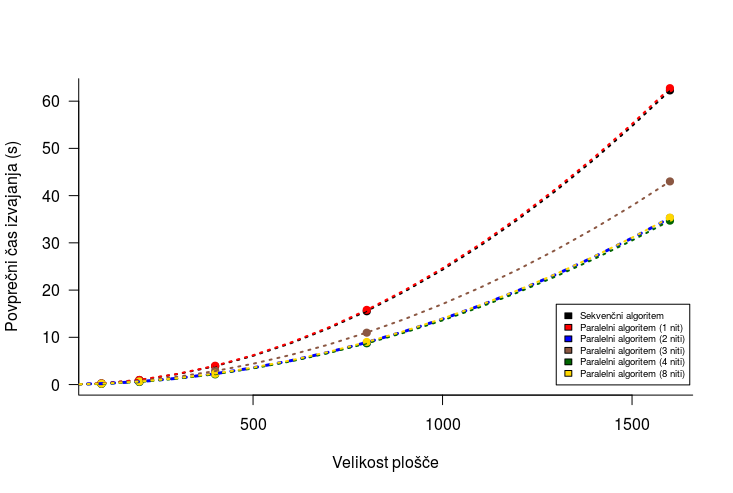
\includegraphics[scale=0.55]{graf-rezultati-3_1.png}
\caption{Povprečni čas izvajanja paralelnega programa glede na velikost plošče ob uporabi različnega števila niti (OpenMP).}
\label{graf-rezultati-3}
\end{center}
\vspace{-25pt}
\end{figure}

Za eno od plošč sva za različna števila niti izračunala faktor pohitritve po enačbi \ref{enacba-faktor-pohitritve}. Največja pohitritev (1,777-krat) je bila dosežena z uporabo štirih niti (toliko je tudi logičnih jeder). Vse vrednosti so grafično predstavljene na sliki \ref{graf-rezultati-pohitritev-3}, razlaga posameznih vrednosti pa je na voljo v poglavju \ref{poglavje-rezultati-2}, kjer so opisani popolnoma skladni rezultati paralelizacije programa s knjižnico Pthreads.

\begin{figure}[H]
\begin{center}
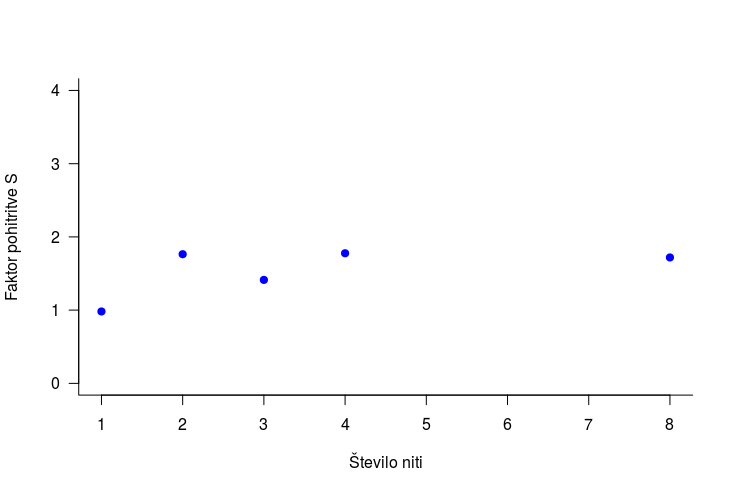
\includegraphics[scale=0.55]{graf-rezultati-3_2.png}
\caption{Faktor pohitritve v odvisnosti od števila uporabljenih niti za fiksno velikost plošče 800$\times$800 (OpenMP).}
\label{graf-rezultati-pohitritev-3}
\end{center}
\vspace{-25pt}
\end{figure}

Po enačbi \ref{enacba-ucinkovitost} sva izračunala še učinkovitost v odvisnosti od števila niti, rezultati pa so vidni na sliki \ref{graf-rezultati-ucinkovitost-3}. Učinkovitost v primeru ene niti je bila tokrat 0,982, v primeru dveh niti pa 0,882. Ostale vrednosti so bistveno nižje, saj ima testni sistem le dve fizični jedri (rezultati so spet skladni s tistimi iz poglavja \ref{poglavje-rezultati-2}, kar je zaradi enake ideje paralelizacije popolnoma smiselno). 

\begin{figure}[H]
\begin{center}
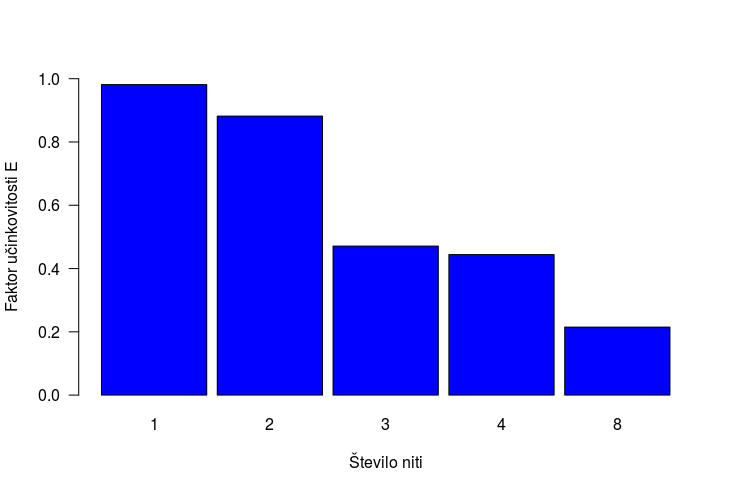
\includegraphics[scale=0.55]{graf-rezultati-3_3.png}
\caption{Učinkovitost v odvisnosti od števila uporabljenih niti za fiksno velikost plošče 800$\times$800 (OpenMP).}
\label{graf-rezultati-ucinkovitost-3}
\end{center}
\vspace{-25pt}
\end{figure}

\pagebreak

\section{Paralelizacija s knjižnico ``OpenCL''}
\label{poglavje-opencl}

\subsection{Ideja paralelizacije}

Algoritem, pripravljen s knjižnico OpenCL je sestavljen iz dveh delov. En del se izvaja na gostitelju (CPE), drugi pa na napravi, ki je podprta z OpenCL platformo (v našem primeru je to GPE).

Program, ki se bo izvajal na napravi, je opisan kot procedura, ki se bo izvedla za posamezen delovni element (angl. work-item). Pri problemu temperaturne plošče nam delovni element predstavlja enkratno računanje nove temperature za eno od točk na plošči, postopek pa je sledeč. Najprej se na podlagi globalnega indeksa delovnega elementa preveri, če pripadajoča točka leži na notranji strani roba plošče. V takem primeru se iz sosednjih točk druge plošče (ki predstavlja stanje temperaturne plošče v prejšnji iteraciji) izračuna novo temperaturo. Če razlika med novo izračunano temperaturo in prejšnjo temperaturo še vedno presega dano mejo \(\varepsilon\), potem ponastavimo globalno zastavico \textit{all\_difs\_below\_eps} na 0 in s tem signaliziramo, da obstaja vsaj ena točka, ki zahteva še nekaj iteracij računanja (na začetku vsake iteracije gostitelj postavi zastavico na 1, računanje pa se lahko zaključi, če nobena od točk ne ponastavi zastavice na 0).

Preden pa se lahko računanje na napravi sploh začne, mora gostitelj pripraviti okolje. Ta najprej prebere datoteko s programom (\textit{kernel.cl}), ki se bo izvajal na napravi. Nato se opravi poizvedba o razpoložljivih OpenCL platformah in napravah. Za želeno napravo se pripravita kontekst in ukazna vrsta, iz prej prebrane datoteke pa se v okviru konteksta pripravi objekt tipa \textit{cl\_program}. Ta se za izbrano napravo prevede, na koncu pa se pripravi še ščepec (objekt tipa \textit{cl\_kernel}), katerega bomo pozneje poganjali na napravi. Gostitelj poskrbi še za alokacijo in inicializacijo ene plošče v svojem pomnilniku, dve kopiji inicializirane plošče pa pripravi v globalnem pomnilniku naprave (na teh bo naprava računala). Poleg plošč se v globalnem pomnilniku naprave rezervira še mesto za zastavico \textit{all\_difs\_below\_eps}. Za smiseln zagon ščepca potrebujemo še dva argumenta - \textit{local\_item\_size} in \textit{global\_item\_size}. Prvi določa velikost delovne skupine (po koliko delovnih elementov naj se izvaja na eni računski enoti) in je v našem programu definiran kot konstanta \textit{WORKGROUP\_SIZE} (pri določanju te vrednosti moramo biti pozorni na zgornjo mejo, saj je ta odvisna od naprave). Drugi označuje celotno število delovnih elementov in je izračunan na podlagi velikosti plošče in velikosti delovne skupine (število vseh delovnih elementov mora biti večkratnik velikosti delovne skupine, hkrati pa želimo imeti vsaj toliko delovnih elementov kot je vseh točk na plošči). S tem imamo vse pripravljeno za računanje. Gostitelj na začetku vsake iteracije postavi zastavico \textit{all\_difs\_below\_eps} v globalnem pomnilniku naprave na 1, nato požene računanje nove plošče na napravi, zamenja vlogi plošč, poveča števec iteracij in preden začne z novo iteracijo preveri stanje zastavice. Kadar ostane zastavica po računanju temperatur nastavljena na 1, se računanje lahko zaključi. Po zadnji iteraciji se končni rezultat (plošča iz globalnega pomnilnika naprave) prenese v pomnilnik gostitelja, vsi preostali viri pa se počistijo.

\subsection{Rezultati}

Program je bil testiran na sistemu, opisanem v tabeli \ref{tabela-specifikacije}. Splača se omeniti še nekaj podrobnosti o testnem okolju, ki za potrebe prejšnjih testiranj niso bile pomembne:
\begin{itemize}
\item pri testiranju je bila uporabljena verzija 1.2 knjižnice OpenCL,
\item največja dovoljena velikost delovne skupine je na testnem sistemu 1024,
\item velikost snopa na testnem sistemu je 32.
\end{itemize}

Meritve so bile opravljene pri petih različnih velikostih delovne skupine: 32, 256, 300, 512 in 1024. Te velikosti so bile izbrane zato, da bi iz meritev videli, če je vedno smiselno nastaviti kar največjo možno velikost delovne skupine, ali je to odvisno od primera uporabe.

Rezultati meritev so prikazani v tabeli \ref{tabela-rezultati-4} in na grafu na sliki \ref{graf-rezultati-4}.

\begin{figure}[H]
\begin{center}
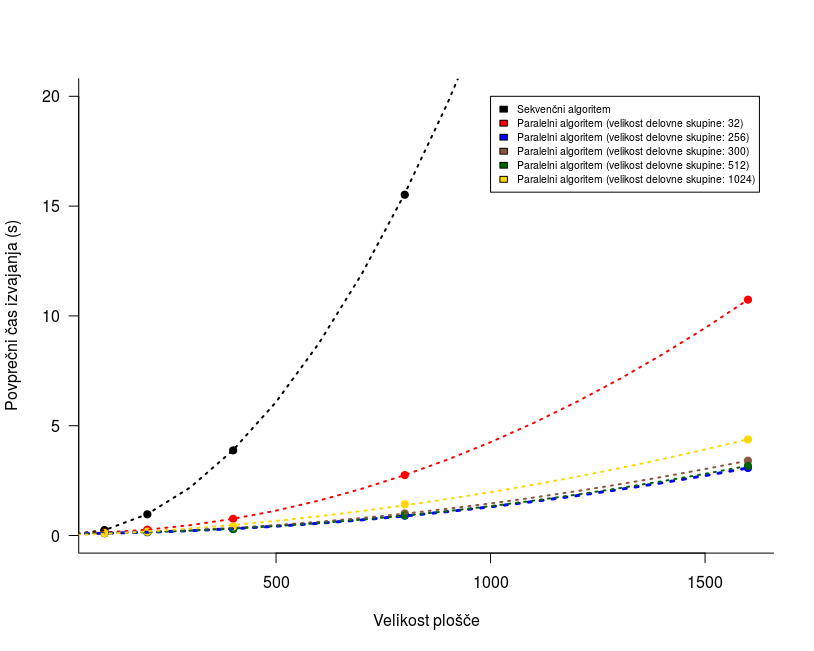
\includegraphics[scale=0.5]{graf-rezultati-4_1.png}
\caption{Povprečni čas izvajanja paralelnega programa glede na velikost plošče ob uporabi različnih velikosti delovne skupine (OpenCL). Graf je zaradi preglednosti ``odrezan" pri povprečnem času izvajanja 20 sekund, zato je potrebno omeniti, da povprečni čas sekvenčnega algoritma izven vidnega monotono narašča in je pri velikosti plošče 1600 enak 62.272 sekund.}
\label{graf-rezultati-4}
\end{center}
\vspace{-25pt}
\end{figure}

\begin{table}[H]
\begin{center}
\caption{Povprečni čas izvajanja paralelnega programa in standardna napaka glede na velikost stranice in velikost delovne skupine pri fiksni meji konvergence $\epsilon = 0.01$ z uporabo knjižnice OpenCL.}
\label{tabela-rezultati-4}
\begin{tabularx}{\textwidth}{|YYYY|}
\hhline{====}
Velikost delovne skupine & Velikost stranice [št. točk] & Povprečni čas izvajanja [s] & Standardna napaka [s] \tabularnewline
\hhline{====}
\multirow{ 5}{*}{32}
& 100 & 0,139 & 0,000 \tabularnewline
& 200 & 0,268 & 0,001 \tabularnewline
& 400 & 0,761 & 0,000 \tabularnewline
& 800 & 2,752 & 0,000 \tabularnewline
& 1600 & 10,738 & 0,001 \tabularnewline
\hline
\multirow{ 5}{*}{256}
& 100 & 0,111 & 0,000 \tabularnewline
& 200 & 0,151 & 0,000 \tabularnewline
& 400 & 0,290 & 0,000 \tabularnewline
& 800 & 0,903 & 0,001 \tabularnewline
& 1600 & 3,074 & 0,000 \tabularnewline
\hline
\multirow{ 5}{*}{300}
& 100 & 0,105 & 0,000 \tabularnewline
& 200 & 0,161 & 0,000 \tabularnewline
& 400 & 0,332 & 0,001 \tabularnewline
& 800 & 1,005 & 0,000 \tabularnewline
& 1600 & 3,407 & 0,000 \tabularnewline
\hline
\multirow{ 5}{*}{512}
& 100 & 0,107 & 0,000 \tabularnewline
& 200 & 0,155 & 0,000 \tabularnewline
& 400 & 0,296 & 0,000 \tabularnewline
& 800 & 0,916 & 0,000 \tabularnewline
& 1600 & 3,171 & 0,000 \tabularnewline
\hline
\multirow{ 5}{*}{1024}
& 100 & 0,110 & 0,000 \tabularnewline
& 200 & 0,176 & 0,000 \tabularnewline
& 400 & 0,413 & 0,000 \tabularnewline
& 800 & 1,420 & 0,000 \tabularnewline
& 1600 & 4,373 & 0,000 \tabularnewline
\hhline{====}
\end{tabularx}
\end{center}
\vspace{-25pt}
\end{table}

\pagebreak

Kot je bilo pričakovano, je algoritem, paraleliziran na grafični kartici, pri vseh preizkušenih velikostih delovne skupine boljši (doseže krajši povprečni čas izvajanja) kot sekvenčni algoritem. Pri manjših velikostih plošče je dosežena pohitritev sicer nekoliko nižja kot bi si mogoče želeli, ampak je bilo to pričakovano, saj je v tem primeru relativno malo računanja glede na vso potrebno režijo, grafične kartice pa svojo moč pokažejo predvsem pri računsko zahtevnih opravilih. To dokazujejo tudi rezultati na večjih dimenzijah plošče. Največja dosežena pohitritev glede na sekvenčni algoritem je bila dosežena pri dimenziji plošče 1600 $\times$ 1600 - sekvenčni algoritem je v povprečju za ta izračun potreboval 62,272 sekund, paralelni algoritem na grafični kartici pa pri najboljši nastavitvi velikosti delovne skupine zgolj 3,074 sekunde.

Slika \ref{graf-rezultati-pohitritev-4} prikazuje faktor pohitritve (določen z enačbo \ref{enacba-faktor-pohitritve}) v odvisnosti od velikosti delovne skupine. Največja pohitritev je bila dosežena pri velikosti delovne skupine 256 (približno \textbf{17}-kratna), najmanjša pa pri velikosti delovne skupine 32 (približno \textbf{6}-kratna).

\begin{figure}[H]
\begin{center}
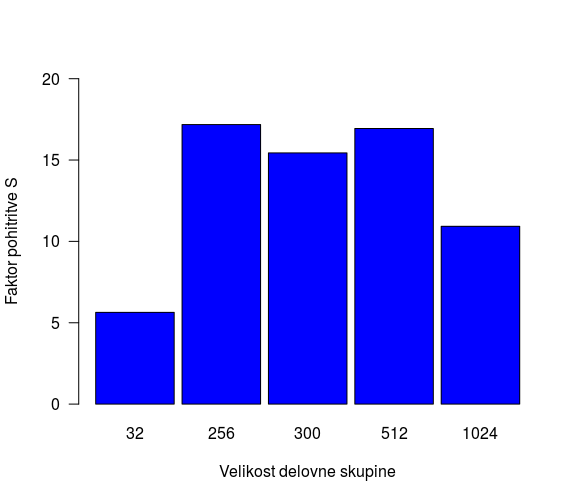
\includegraphics[scale=0.55]{graf-rezultati-4_2.png}
\caption{Faktor pohitritve pri različnih velikostih delovne skupine ter fiksni velikosti plošče 800$\times$800 (OpenCL).}
\label{graf-rezultati-pohitritev-4}
\end{center}
\vspace{-25pt}
\end{figure}

Iz rezultatov je vidno, da nastavljanje velikosti delovne skupine na največjo možno velikost ni nujno najboljša ideja. Najkrajši povprečni časi izvajanja namreč niso bili izmerjeni pri velikosti plošče 1024 (kolikor je največja dovoljena velikost skupine na grafični kartici na testnem sistemu), pač pa pri velikosti skupine 256. Izjema je zgolj velikost temperaturne plošče 100 $\times$ 100, kjer pa je izmerjeni povprečni čas nekaj tisočink sekunde večji od najboljšega. OpenCL omogoča tudi možnost, da ne določimo velikosti skupine eksplicitno, pač pa pustimo, da se ta določi samodejno, vendar s tem nisva nič pridobila. Časi so bili približno enaki, nekje pa celo slabši kot pri ročno nastavljeni velikosti delovne skupine 256. Za najboljše rezultate, je torej bolje eksperimentalno določiti velikost delovne skupine kot pa se zanašati, da bo sistem res našel najboljšo nastavitev.

Posebno zanimive so še meritve pri velikosti delovne skupine 300. Kljub temu, da je velikost delovne skupine večja, sistem pri teh nastavitvah za skoraj vse testirane dimenzije plošče doseže slabše rezultate kot pri velikosti delovne skupine 256. Razlog za to je, da mora biti velikost delovne skupine za optimalno izkoriščanje virov večkratnik velikosti snopa. Še en razlog za slabše dosežene povprečne čase je bil opisan v prejšnjem odstavku (večanje velikosti delovne skupine ne prinese nujno krajšega časa izvajanja).

Za konec pa poglejmo še, kako dobro se je algoritem, paraleliziran na grafični kartici, obnesel v primerjavi s prejšnjimi metodami paralelizacije (več o načinu paralelizacije s knjižnicama Pthreads in OpenMP je napisano v poglavjih \ref{poglavje-pthreads} in \ref{poglavje-openmp}). Na sliki \ref{graf-rezultati-primerjava-4} so prikazani povprečni časi izvajanja za različne velikosti temperaturne plošče, doseženi z različnimi načini paralelizacije. Za boljšo predstavo o doseženih izboljšavah so na grafu tudi povprečni časi, doseženi s sekvenčnim algoritmom. Paralelizacija na grafični kartici doseže tako v najboljšem kot tudi v najslabšem primeru krajše povprečne čase izvajanja kot vsi prejšnji poizkusi paralelizacije. Temu je tako, ker ima naš problem visoko stopnjo podatkovnega paralelizma (z dovolj velikim številom računskih enot bi lahko tudi celotno ploščo izračunali v enem koraku), to je pa posebej ugodno za paralelizacijo z grafično kartico.

\begin{figure}[H]
\begin{center}
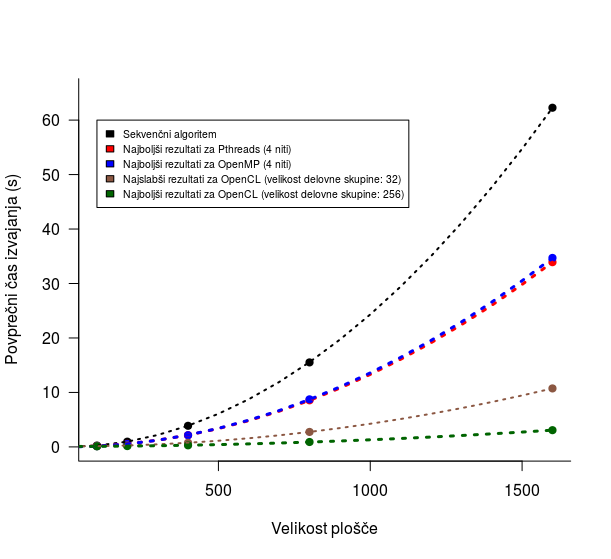
\includegraphics[scale=0.7]{graf-rezultati-4_1_1.png}
\caption{Primerjava povprečnih časov izvajanja sekvenčnega algoritma in različnih verzij paralelnega algoritma pri različnih dimenzijah temperaturne plošče.}
\label{graf-rezultati-primerjava-4}
\end{center}
\vspace{-25pt}
\end{figure}

\pagebreak

\section{Paralelizacija s knjižnico ``OpenMPI''}
\label{poglavje-mpi}

\subsection{Ideja paralelizacije}

Paralelni programi, pripravljeni s knjižnico OpenMPI, se v celoti izvajajo vzporedno (ob zagonu navedemo želeno število procesov). Delitev dela je organizirana na podlagi identifikacijskih številk procesov, na enak način pa lahko po potrebi poskrbimo še za vejitve, če želimo, da eden od procesov deluje kot gospodar.

V našem primeru temperaturne plošče smo se odločili, da procese navidezno razporedimo v mrežo \(\sqrt{p} \: \times \sqrt{p}\), vsakemu pa se dodeli pripadajoč blok plošče. Takšna delitev dela zahteva (v primerjavi z delitvijo na vodoravne pasove) nekoliko več organizacije pri izmenjevanju robov plošče, vendar se v celoti gledano pošilja manjša količina podatkov. Za ploščo velikosti \(s \times s\) in \(p\) procesov se izkaže, da pri delitvi na pasove izmenjamo \(2 \cdot s \cdot (p-1)\) točk na iteracijo, z mrežo blokov pa izmenjamo le \(4 \cdot s \cdot (\sqrt{p}-1)\) točk na iteracijo, kar prinese pri večjem številu procesov kar veliko razliko. Po drugi strani nas takšna delitev rahlo omejuje, saj lahko izkoristimo le toliko virov, za kolikor se takšna delitev izide (1, 2, 4, 9, 16...). V programu zato takoj na začetku obdržimo le \(\left \lfloor{\sqrt{p}}\right \rfloor ^ 2\) procesov.

Na vsakem od obdržanih procesov se nato pripravita dve celotni plošči, za tem pa se izračunajo še meje, v katerih bo dan proces računal. Taka rešitev je sicer precej pomnilniško potratna (vsak proces ima shranjeno celotno ploščo, potrebuje pa le svoj del), ampak se je v praksi izkazala za boljšo kot npr. inicializacija plošče na enem procesu in pošiljanje delov plošče med ostale ali pa porazdeljena inicializacija delov plošče (naša implementacija inicializacije namreč vsebuje nekaj odvisnosti med sosednjimi točkami, kar prinese potrebo po dodatni komunikaciji med procesi).

V tej točki je vse pripravljeno in začnemo z računanjem. Vsak proces izračuna svoj del in lokalno največjo izračunano razliko. Za tem se opravi skupna redukcija, kjer kot rezultat vsak proces dobi globalno maksimalno razliko (ko je ta dovolj majhna se zaključi računanje), hkrati pa ta ukaz služi tudi kot prepreka na kateri se procesi časovno sinhronizirajo. Zabeležimo še novo število iteracij in zamenjamo vlogi plošč, za tem pa sledi izmenjevanje robov. Vsak proces najprej neblokirajoče pošlje robove vsem sosedom, nato pa blokirajoče prejema želene podatke. Takoj, ko posamezen proces prejme vse podatke, lahko brez prepreke nadaljuje z računanjem naslednje iteracije, po računanju pa se procesi zaradi skupne redukcije spet sinhronizirajo. Proces izmenjevanja robov, bi lahko zaradi velikih stroškov vzpostavljanja komunikacije izboljšali tako, da bi izmenjali širši rob, nato pa bi nekaj iteracij računali brez izmenjave robov (v takem primeru bi sicer imeli nekaj več računanja, ampak je to cenejše od komunikacije).

Ob koncu se izračunane dele plošče pošlje iz posameznih procesov na prvega (gospodar), ta pa podatke sprejme, organizira v celoto in nato ploščo shrani kot datoteko. Za tem procesi le še počistijo rezerviran pomnilnik.

\subsection{Rezultati}

\subsubsection{Rezultati na lokalnem testnem sistemu}

Program smo lokalno testirali na enakem testnem sistemu kot pri prejšnjih testiranjih (specifikacije so navedene v tabeli \ref{tabela-specifikacije}), rezultati meritev pa so predstavljeni v tabeli \ref{tabela-rezultati-5}.

Za lažjo primerjavo smo meritve časov opravili za popolnoma enak nabor parametrov kot pri testiranju s knjižnicama Pthreads in OpenMP, vendar je tukaj pomembno dejstvo, da se program zaradi posebne delitve dela vedno izvaja le na \(\left \lfloor{\sqrt{p}}\right \rfloor ^ 2\) procesih (p je zahtevano število procesov). V tabeli \ref{tabela-rezultati-5} smo zato poleg zahtevanega števila procesov navedli še število aktivnih procesov za primere, ko se ti dve števili razlikujeta.

Smiselno lahko torej obravnavamo le primere, kjer smo zahtevali 1 in 4 procese. Ti rezultati so zelo podobni rezultatom, ki smo jih pri enakih parametrih dobili s paralelizacijo s knjižnicama Pthreads in OpenMP, kar je bilo tudi pričakovano. Medprocesna komunikacija znotraj enega vozlišča je pri MPI najverjetneje implementirana kar z uporabo deljenega pomnilnika in je zato časovna zakasnitev pri izmenjevanju robov zelo majhna.

Pri ostalih primerih (2, 3 in 8 zahtevainh procesov) so izmerjeni časi seveda primerljivi s časi meritev, pri katerih smo že sami zahtevali toliko procesov, kolikor jih je bilo pri računanju dejansko aktivnih. Nekaj več časa se je očitno porabilo le na račun upravljanja z dodatnimi neaktivnimi procesi.

\begin{table}[H]
\begin{center}
\caption{Povprečni čas izvajanja paralelnega programa (na lokalnem testnem sistemu) in standardna napaka glede na velikost stranice in število uporabljenih procesov z uporabo knjižnice OpenMPI.}
\label{tabela-rezultati-5}
\begin{tabularx}{\textwidth}{|YYYY|}
\hhline{====}
Število uporabljenih procesov & Velikost stranice [št. točk] & Povprečni čas izvajanja [s] & Standardna napaka [s] \tabularnewline
\hhline{====}
\multirow{ 5}{*}{1}
& 100 & 0,312 & 0,000 \tabularnewline
& 200 & 1,040 & 0,004 \tabularnewline
& 400 & 3,961 & 0,013 \tabularnewline
& 800 & 15,547 & 0,013 \tabularnewline
& 1600 & 65,138 & 0,104 \tabularnewline
\hline
\multirow{ 5}{*}{2 (1)}
& 100 & 0,350 & 0,000 \tabularnewline
& 200 & 1,153 & 0,003 \tabularnewline
& 400 & 4,393 & 0,004 \tabularnewline
& 800 & 17,424 & 0,014 \tabularnewline
& 1600 & 72,692 & 0,044 \tabularnewline
\hline
\multirow{ 5}{*}{3 (1)}
& 100 & 0,357 & 0,000 \tabularnewline
& 200 & 1,162 & 0,003 \tabularnewline
& 400 & 4,400 & 0,004 \tabularnewline
& 800 & 17,432 & 0,016 \tabularnewline
& 1600 & 72,757 & 0,074 \tabularnewline
\hline
\multirow{ 5}{*}{4}
& 100 & 0,219 & 0,000 \tabularnewline
& 200 & 0,603 & 0,000 \tabularnewline
& 400 & 2,140 & 0,000 \tabularnewline
& 800 & 8,388 & 0,003 \tabularnewline
& 1600 & 34,598 & 0,012 \tabularnewline
\hline
\multirow{ 5}{*}{8 (4)}
& 100 & 0,302 & 0,000 \tabularnewline
& 200 & 0,723 & 0,000 \tabularnewline
& 400 & 2,417 & 0,004 \tabularnewline
& 800 & 9,316 & 0,016 \tabularnewline
& 1600 & 38,208 & 0,072 \tabularnewline
\hhline{====}
\end{tabularx}
\end{center}
\vspace{-25pt}
\end{table}

\pagebreak
\subsubsection{Rezultati na omrežju grid}

Program, paraleliziran s knjižnico OpenMPI, sva testirala tudi na omrežju grid, ki ga upravlja konzorcij SLING (slovenska iniciativa za nacionalni grid). \\
Ta uporabnikom omogoča preprost dostop do razpršenega omrežja računskih virov za namen paralelnega računanja in obdelave podatkov. Iniciativo vodi Arnes, med člani skupine SLING pa so še organizacije, kot so Institut Jožef Stefan, Agencija republike Slovenije za okolje, Comtrade, itd..

Program sva testirala na 4, 16, 25 in 64 jedrih. Več kot s 64 jedri programa nisva testirala predvsem zato, ker se čas čakanja na dodelitev virov na gridu močno poveča, če zahtevamo več virov. Rezultati testiranja so vidni v tabeli \ref{tabela-rezultati-5-sling} in na sliki \ref{graf-rezultati-5}.

Vidno je, da za majhno velikost plošče večje število procesov doseže slabše rezultate kot manjše število procesov. Razlog je v tem, da z večanjem števila procesov povečujemo čas komunikacije med procesi, količina računanja pa ostaja enaka.
Prejšnjo poved dokazuje dejstvo, da se nam pri večjih dimenzijah plošče uporaba večjega števila procesov obrestuje (do neke meje) - primer tega je čas izvajanja za velikost plošče $1600 \times 1600$, kjer je čas izvajanja z uporabo 16 in 25 procesov krajši kot tisti z uporabo 4 procesov.

\begin{table}[H]
\begin{center}
\caption{Povprečni čas izvajanja paralelnega programa (na omrežju SLING) in standardna napaka glede na velikost stranice in število uporabljenih procesov z uporabo knjižnice OpenMPI.}
\label{tabela-rezultati-5-sling}
\begin{tabularx}{\textwidth}{|YYYY|}
\hhline{====}
Število uporabljenih procesov & Velikost stranice [št. točk] & Povprečni čas izvajanja [s] & Standardna napaka [s] \tabularnewline
\hhline{====}
\multirow{ 5}{*}{4}
& 100 & 0,352 & 0,003 \tabularnewline
& 200 & 0,717 & 0,009 \tabularnewline
& 400 & 1,483 & 0,011 \tabularnewline
& 800 & 4,394 & 0,038 \tabularnewline
& 1600 & 23,611 & 0,045 \tabularnewline
\hline
\multirow{ 5}{*}{16}
& 100 & 0,473 & 0,013 \tabularnewline
& 200 & 0,702 & 0,001 \tabularnewline
& 400 & 0,932 & 0,015 \tabularnewline
& 800 & 2,479 & 0,018 \tabularnewline
& 1600 & 8,661 & 0,024 \tabularnewline
\hline
\multirow{ 5}{*}{25}
& 100 & 0,858 & 0,053 \tabularnewline
& 200 & 0,855 & 0,001 \tabularnewline
& 400 & 0,788 & 0,018 \tabularnewline
& 800 & 2,094 & 0,062 \tabularnewline
& 1600 & 7,601 & 0,053 \tabularnewline
\hline
\multirow{ 5}{*}{64}
& 100 & 32,383 & 0,131 \tabularnewline
& 200 & 32,483 & 0,092 \tabularnewline
& 400 & 31,955 & 0,052 \tabularnewline
& 800 & 32,432 & 0,126 \tabularnewline
& 1600 & 33,325 & 0,083 \tabularnewline
\hhline{====}
\end{tabularx}
\end{center}
\vspace{-25pt}
\end{table}

\begin{figure}[H]
\begin{center}
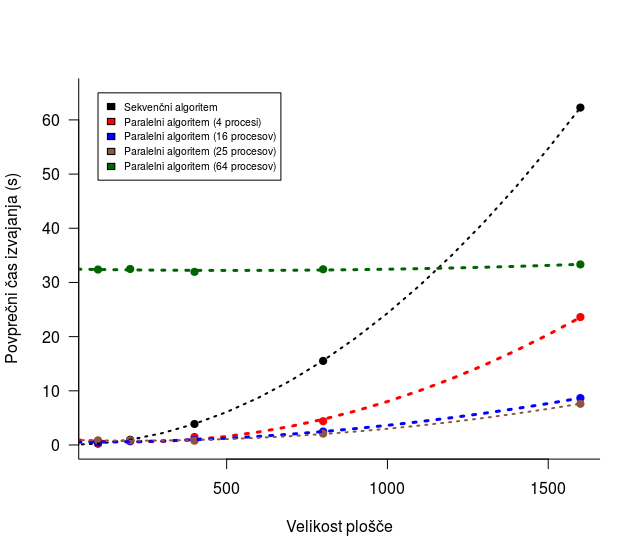
\includegraphics[scale=0.6]{graf-rezultati-5_1.png}
\caption{Povprečni čas izvajanja paralelnega programa in standardna napaka glede na velikost stranice in število uporabljenih procesov pri fiksni meji konvergence $\epsilon = 0.01$ z uporabo knjižnice OpenMPI.}
\label{graf-rezultati-5}
\end{center}
\vspace{-25pt}
\end{figure}

Za ploščo velikosti \(800 \times 800\) smo izračunali faktor pohitritve (enačba \ref{enacba-faktor-pohitritve}) za različna števila procesov (vidno na grafu \ref{graf-rezultati-pohitritev-5}). Pohitritev najprej z večanjem števila procesov narašča, nato pa strmo pade, ko prečkamo mejo 32 - toliko je namreč procesorskih jeder na enem od vozlišč v omrežju. Ko mejo prečkamo, pridobimo velik časovni pribitek zaradi visoke latence pri komunikaciji med procesi. To je še lepše prikazano na grafu \ref{graf-rezultati-5}, kjer je vidno, da časovni pribitek ni v veliki meri odvisen od velikosti plošče (od skupne količine podatkov, ki se med računanjem prenaša), ampak je pretežno odvisen od števila zaporednih začetkov prenosa (torej od števila iteracij, ki je v našem primeru približno konstantno za vse velikosti plošče pri fiksnem epsilonu). Vidimo torej, da bi se nam za računanje na omrežju v veliki meri izplačalo implementirati že prej predlagan postopek izmenjevanja nekoliko širšega roba. Tako smo najboljši rezultat dosegli s tem, da smo prenose obdržali na lokalnem nivoju in za 25 procesov dosegli 7,410-kratno pohitritev (25 je namreč največje število, ki ni večje od 32 in ima za koren celo število).

\begin{figure}[H]
\begin{center}
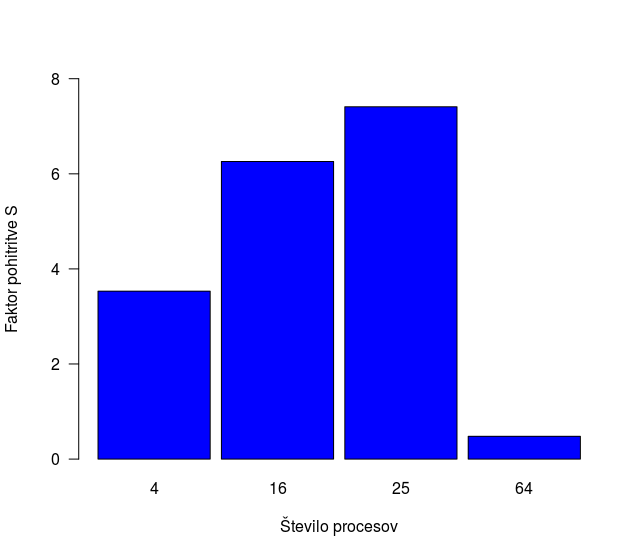
\includegraphics[scale=0.5]{graf-rezultati-5_2.png}
\caption{Faktor pohitritve v odvisnosti od števila uporabljenih procesov za fiksno velikost plošče 800$\times$800 (OpenMPI).}
\label{graf-rezultati-pohitritev-5}
\end{center}
\vspace{-25pt}
\end{figure}

Prej izračunane faktorje pohitritve smo preračunali (enačba \ref{enacba-ucinkovitost}) še v učinkovitost. Največja učinkovitost (0,883) je bila dosežena pri najmanjšem številu pognanih procesov. Iz grafa na sliki \ref{graf-rezultati-ucinkovitost-5} se lepo vidi, da z večanjem števila uporabljenih procesov večamo stroške komunikacije, kar pri fiksni velikosti plošče (kjer je količina računanja vedno enaka) pomeni nižjo učinkovitost na posamezen proces. Ta problem je najlažje rešiti tako, da ob večanju procesov poskušamo latenco prikriti s tem, da poleg tega tudi več računamo (torej povečamo velikost plošče).

\begin{figure}[H]
\begin{center}
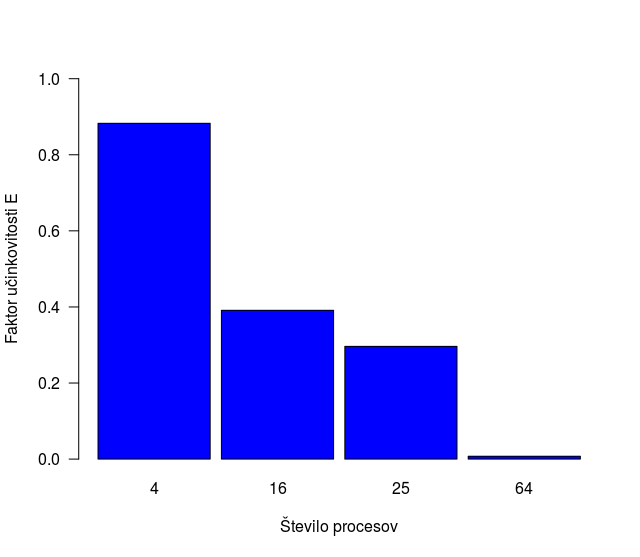
\includegraphics[scale=0.5]{graf-rezultati-5_3.png}
\caption{Učinkovitost v odvisnosti od števila uporabljenih procesov za fiksno velikost plošče 800$\times$800 (OpenMPI).}
\label{graf-rezultati-ucinkovitost-5}
\end{center}
\vspace{-25pt}
\end{figure}

\section{Pregled uporabljenih metod paralelizacije}

V posameznih poglavjih so bile opisane posamezne metode paralelizacije, to poglavje pa združuje najboljše dosežene rezultate. Graf na sliki \ref{graf-rezultati-pregled-6} prikazuje čas izvajanja sekvenčnega algoritma ter najboljše dosežene čase izvajanja s posameznimi pristopi paralelizacije.

\begin{figure}[H]
\begin{center}
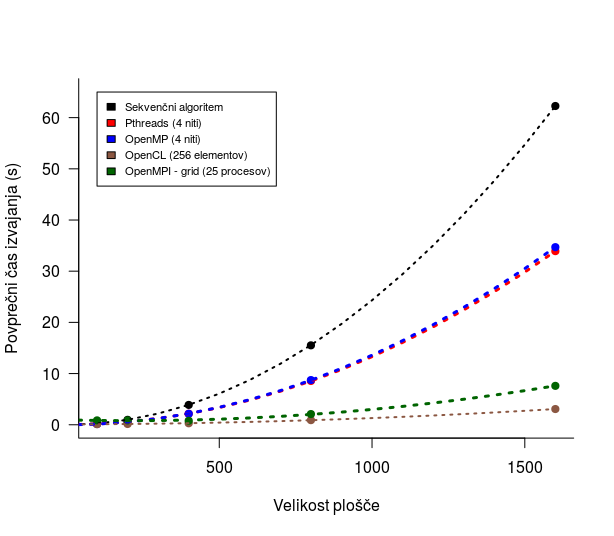
\includegraphics[scale=0.7]{graf-rezultati-6-pregled.png}
\caption{Čas izvajanja sekvenčnega algoritma ter najboljši (najkrajši) doseženi časi izvajanja s posameznimi pristopi paralelizacije.}
\label{graf-rezultati-pregled-6}
\end{center}
\vspace{-25pt}
\end{figure}

Pri majhnih velikostih plošče (konkretno je najmanjša velikost plošče, za katero so bile opravljene meritve, tukaj $100 \times 100$) so si (povprečni) časi izvajanja precej podobni. To je posledica dejstva, da je tukaj relativno malo računanja v primerjavi s potrebno režijo za vzpostavitev paralelizacije. Zato paralelni programi ves tisti čas, ki so ga pridobili na račun paralelnega izvajanja, izgubijo zaradi režije. Poleg tega je povprečni čas izvajanja pri majhnih velikostih plošče že v primeru sekvenčnega algoritma precej kratek (približno 0,250 sekunde), zato izboljšave niso tako očitne. Najkrajši povprečni čas izvajanja doseže paralelizacija s knjižnico OpenCL, 0,111 sekunde.

Z večanjem velikosti plošče povprečni čas izvajanja hitro narašča (kvadratno v odvisnosti od velikosti stranice). Tukaj se začnejo kazati prednosti uporabe paralelnih pristopov. Kot primer velja omeniti, da pri velikosti plošče $1600 \times 1600$ sekvenčni algoritem rabi v povprečju 62,272 sekund, paralelni algoritem na grafični kartici (paraleliziran s pomočjo OpenCL) pa zgolj 3,074 sekunde. Naraščanje faktorja pohitritve z večanjem plošče se še lepše vidi na sliki \ref{graf-rezultati-pohitritve-pregled-6}.

\begin{figure}[H]
\begin{center}
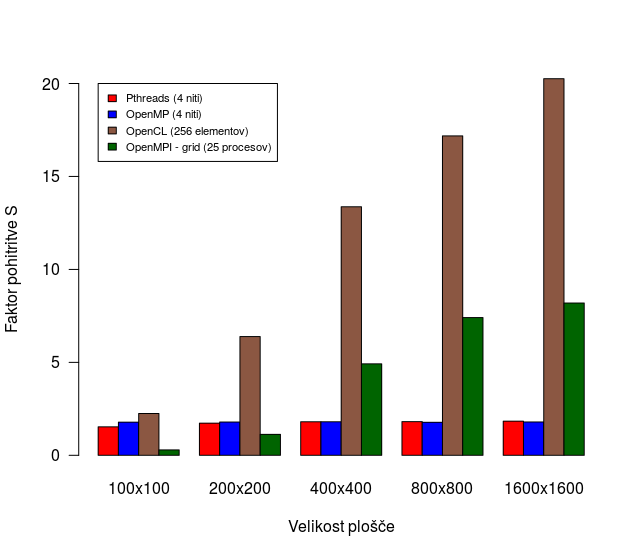
\includegraphics[scale=0.7]{graf-rezultati-6_1-pregled.png}
\caption{Faktor pohitritve, dosežen s posameznimi pristopi paralelizacije za različne velikosti plošče.}
\label{graf-rezultati-pohitritve-pregled-6}
\end{center}
\vspace{-25pt}
\end{figure}

Izmed uporabljenih pristopov paralelizacije sta si paralelizacija s knjižnico Pthreads in paralelizacija s knjižnico OpenMP zelo podobni - povprečni časi izvajanja so si zelo blizu, iz tega pa sledi, da so si tudi pohitritve zelo podobne. Majhne razlike so najverjetneje posledica različno učinkovitih implementacij paralelnih konstruktov v posameznih knjižnicah.

Najboljše rezultate je za vse (izbrane) velikosti plošče dosegla paralelizacija na grafični kartici (s knjižnico OpenCL). Na $1600 \times 1600$ je dosegla kar 20,258-kratno pohitritev (glede na sekvenčni algoritem). Kljub temu pa to ne pomeni, da bo temu vedno tako - kateri pristop bo deloval najbolje, je močno odvisno od tipa problema. Problem temperaturne plošče ima visoko stopnjo podatkovnega paralelizma in je zato primeren za paralelizacijo na GPE. Če bi naš problem zahteval številne vejitve programskega toka in manj vzporednega računanja, bi pristop z OpenCL dosegel veliko slabše rezultate.

Poleg paralelizacije na grafični kartici, smo precej dobre rezultate dosegli tudi na omrežju grid, kjer smo testirali paralelizacijo s knjižnico MPI. Nekoliko nas je presenetilo dejstvo, da je latenco pri komunikaciji na omrežju zelo težko prikriti. Najboljši rezultat smo namreč dosegli, ko smo število procesov omejili tako, da se je algoritem v celoti izvajal na enem vozlišču. V primeru večjega števila vozlišč se je pri vseh časih pojavil pribitek (približno 30 sekund), so si pa ti časi precej podobni za različne velikosti plošče, kar nakazuje, da bi lahko z ekstremnim večanjem problema dosegli dober rezultat tudi na tak način.

Običajno prav tak pristop (večanje problema) uporabljamo, ko želimo za večje število vzporednih procesov obdržati enako učinkovitost. Veljati mora naslednja zveza:
\begin{equation} \label{enacba-raztegljivost}
T_s(n) \geq C \cdot T_{overhead}(n,p),
\end{equation}
kjer \(T_s(n)\) predstavlja čas, ki ga za izvajanje potrebuje serijski algoritem (v odvisnosti od velikosti problema), \(T_{overhead}(n,p)\) je skupen odvečni čas, ki ga pridobimo s paralelizacijo (v odvisnosti od velikosti problema in števila paralelnih enot), \(C\) je pa konstanta, ki zajema zahtevo po konstantni učinkovitosti. Zgornje čase lahko bolj jasno zapišemo kot:
\begin{equation}
T_s(n) = \sigma(n) + \varphi(n),
\end{equation}
\begin{equation}
T_{overhead}(n,p) = (p-1) \cdot \sigma(n) + p \cdot \kappa(n,p),
\end{equation}
kjer je \(\sigma\) čas izvajanja tistega dela algoritma, ki ga ne moremo paralelizirati, \(\varphi\) čas izvajanja dela algoritma, ki ga lahko paraleliziramo in \(\kappa\) dodaten čas, potreben za komunikacijo in sinhronizacijo med paralelnimi procesi. \\
V našem primeru bomo za velikost problema uporabili kar velikost stranice plošče, število iteracij pa naj bo konstantno. Na ta način lahko iz obravnave izpustimo še del algoritma, kjer se plošča inicializira, razdeli med procese in na koncu spet združi. Delež časa, ki se porabi za to, lahko namreč enostavno približamo k 0 s tem, ko povečamo zahtevano število iteracij (\(\varepsilon \to 0\)). To si lahko privoščimo, saj ob tem nimamo nobenih dodatnih pomnilniških zahtev. Če torej upoštevamo le del algoritma, kjer ponavljajoče računamo temperature, bo veljalo naslednje:
\begin{equation}
\sigma(n) = O(0),
\end{equation}
\begin{equation}
\varphi(n) = O(n^2),
\end{equation}
\begin{equation}
\kappa(n,p) = O(\frac{n}{\sqrt{p}} + \log{p}).
\end{equation}
V enačbi \ref{enacba-raztegljivost} lahko zdaj uporabimo zgornje časovne zahtevnosti in dobimo naslednjo zvezo:
\begin{equation}
n^2 \geq C \cdot (n \sqrt{p} + p \log{p}).
\end{equation}
Iz te lahko izpeljemo pogoj, ki nam pove, vsaj kakšna naj bo nova velikost problema, če želimo ob večanju števila paralelnih enot obdržati enako učinkovitost:
\begin{equation}
n^2 - c \sqrt{p} \cdot n - C p \log{p} \geq 0,
\end{equation}
\begin{equation}
n \leq \frac{C \sqrt{p} - \sqrt{C^2 p + 4 C p \log{p}}}{2} \quad \textrm{ali} \quad n \geq \frac{C \sqrt{p} + \sqrt{C^2 p + 4 C p \log{p}}}{2}.
\end{equation}
Izkaže se, da lahko za naše potrebe prvi del pogoja izpustimo, saj nam ta k rešitvi nikoli ne doda takih \(n\)-jev, ki bi bili večji ali enaki 1, zanimajo pa nas le ti. Tako dobimo naslednjo zahtevo:
\begin{equation}
n \geq f(p) \quad \textrm{za} \quad f(p) = \frac{C \sqrt{p} + \sqrt{C^2 p + 4 C p \log{p}}}{2},
\end{equation}
radi pa bi izvedeli še kakšnega reda bo pomnilniška zahtevnost za posamezno paralelno enoto (v odvisnosti od \(p\)). V našem primeru poznamo odvisnost od velikosti problema:
\begin{equation}
M(n) = O(n^2),
\end{equation}
iz te pa sledi:
\begin{equation}
M(f(p)) = O(p \log{p}).
\end{equation}
To pomeni, da sistem ni popolnoma raztegljiv, saj moramo z večanjem števila procesov (ob želji, da dosežemo enako učinkovitost) toliko povečati velikost problema, da nam narašča tudi pomnilniška zahtevnost na posamezni procesni enoti. Na tem mestu lahko spet omenimo, da je tukaj še nekaj prostora za izboljšave, saj ima v naši implementaciji vsak proces shranjeno celotno ploščo (in ne le svoj del), ampak za praktične potrebe ta izboljšava ni bila potrebna. Tudi iz vidika raztegljivosti nam izboljšava ne bi prinesla popolne raztegljivosti, saj bi bila v tem primeru pomnilniška zahtevnost v odvisnosti od števila procesnih enot enaka \(M(f(p)) = O(\log{p})\) in ne konstantna, kot bi si želeli.

\section{Zaključek}

\end{document}
